\chapter{To verify the truth table for NOR gate}

\section{Apparatus}
%\label{sec:objectives}
	\begin{itemize}
		\tightlist
		\item Kit for realization of gates
		\item Connecting Leads
	\end{itemize}

\section{Theory}
	This is a NOT-OR gate which is equal to an OR gate followed by a NOT gate. The outputs of all NOR gates are low if any of the inputs are high. The symbol is an OR gate with a small circle on the output. The small circle represents inversion.
	\begin{figure}[h]
		\centering
		
\includegraphics{img/exp5/1}
		\caption{Symbol for NOR gate}
		\label{fig:5:1}
	\end{figure}
	\begin{figure}[h]
		\centering
		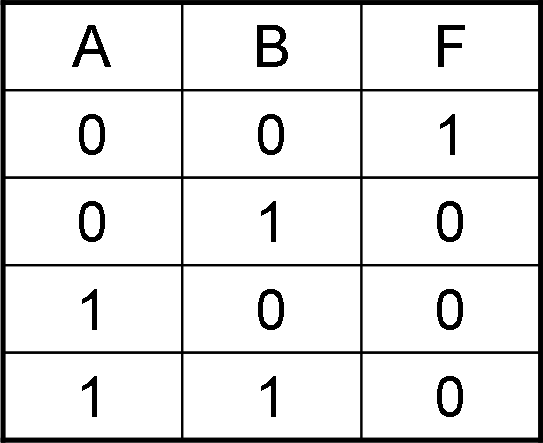
\includegraphics{img/exp5/2}
		\caption{Truth Table for NOR gate}
		\label{fig:5:2}
	\end{figure}
	
	A simple 2-input logic NOR gate can be constructed using RTL (Resistor-transistor-logic) switches connected together as shown below with the inputs connected directly to the transistor bases. Both transistors must be cut-off or “OFF” for an output at Q.
	
	\begin{figure}[h]
		\centering
		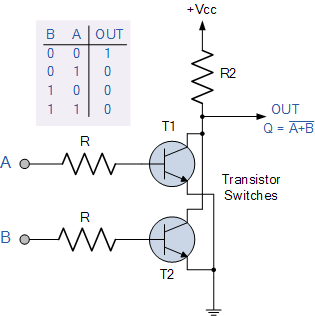
\includegraphics{img/exp5/3}
		\caption{Circut for making NOR gate}
		\label{fig:5:3}
	\end{figure}
				
\section{Procedure}
	\subsubsection{Simulator 1}
	\begin{itemize}
		\tightlist
		\item Connect the supply(+5V) to the circuit.
		\item Press the switches for inputs "A" and "B".
		\item The bulb glows if both the switches are OFF else it won't glow.
		\item Repeat step-2 and step-3 for all state of inputs.
	\end{itemize}

	\subsubsection{Simulator 2}
	\begin{itemize}
		\tightlist
		\item Enter the Boolean input "A" and "B".
		\item Enter the Boolean output for your corresponding inputs.
		\item Click on "Check" Button to verify your output.
		\item Click "Print" if you want to get print out of Truth Table.
	\end{itemize}


\section{Observations}
	\begin{figure}[h]
		\centering
		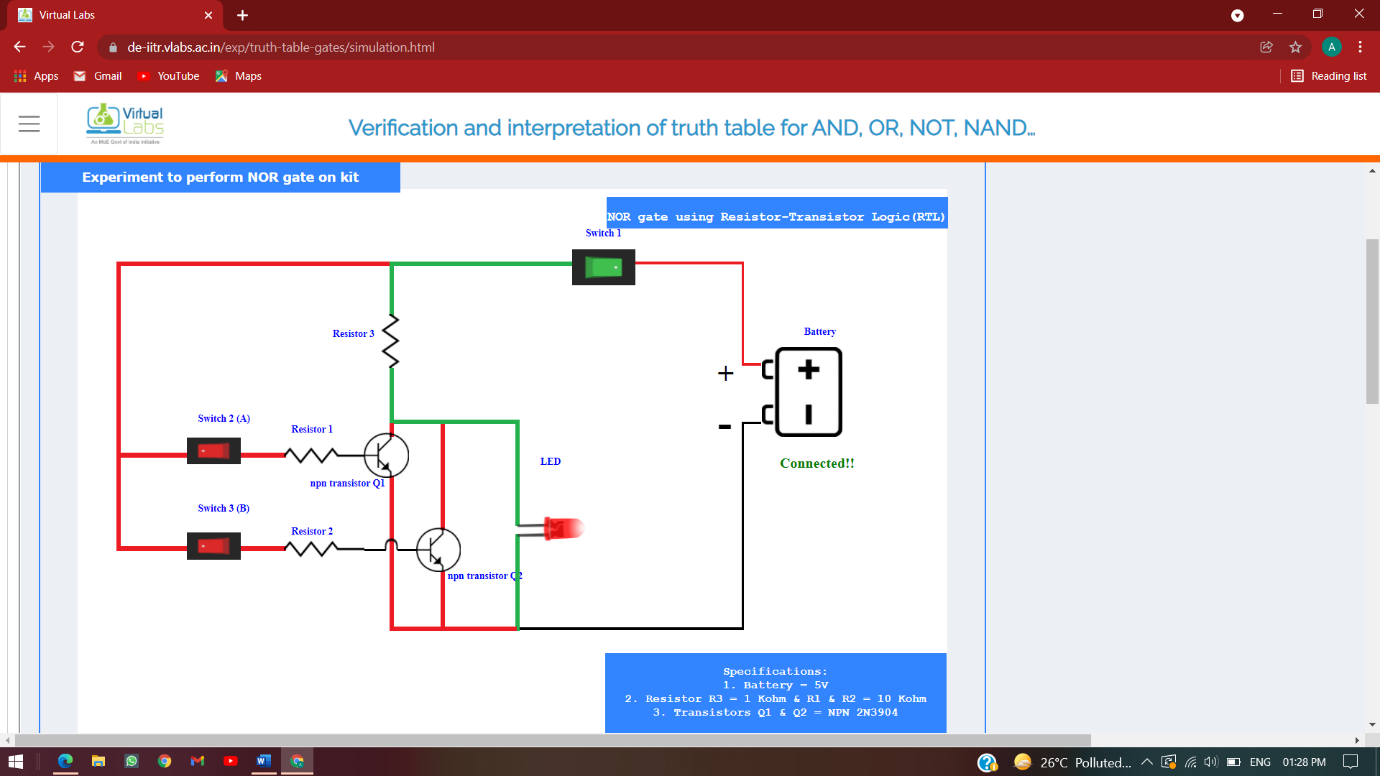
\includegraphics[width=0.9\linewidth]{img/exp5/4}
		\caption{}
		\label{fig:5:4}
	\end{figure}
		\begin{figure}[h]
		\centering
		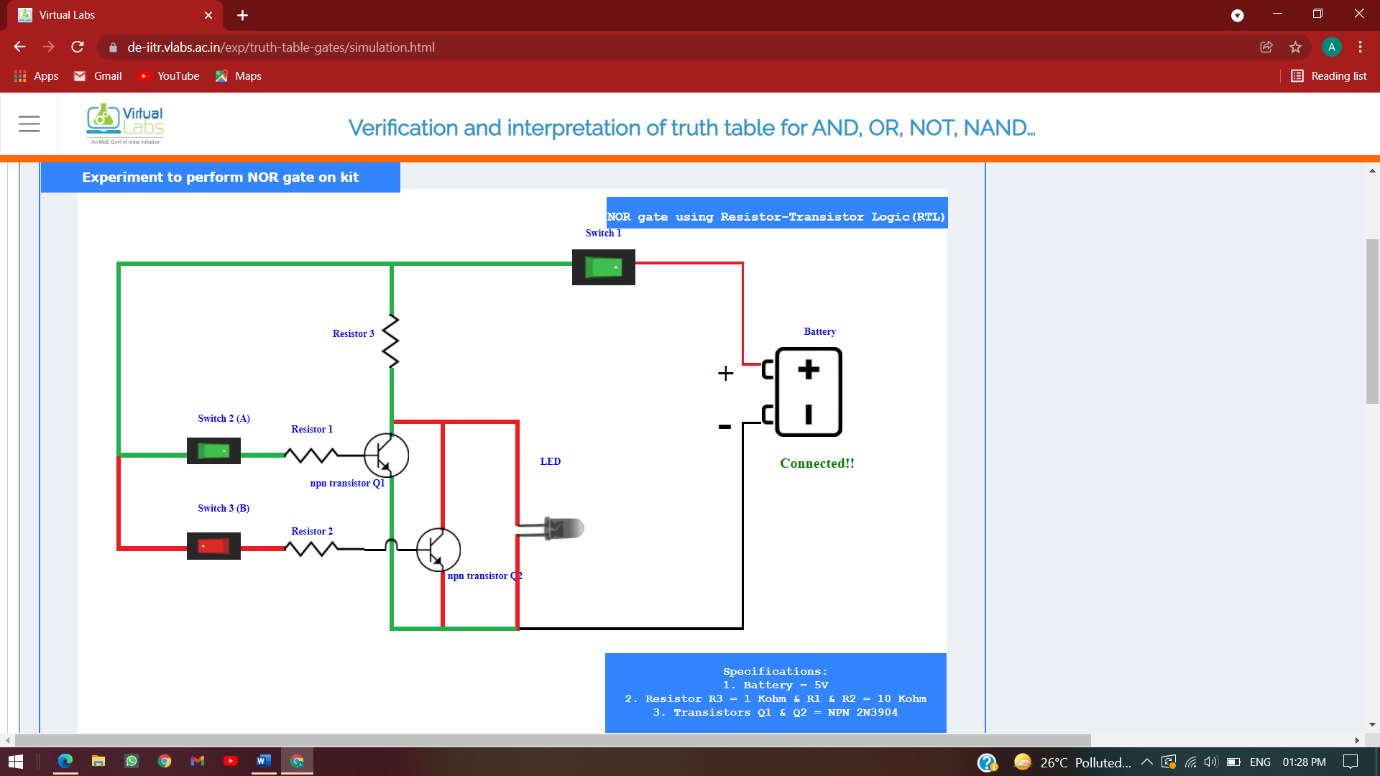
\includegraphics[width=0.9\linewidth]{img/exp5/5}
		\caption{}
		\label{fig:5:5}
	\end{figure}
		\begin{figure}[h]
		\centering
		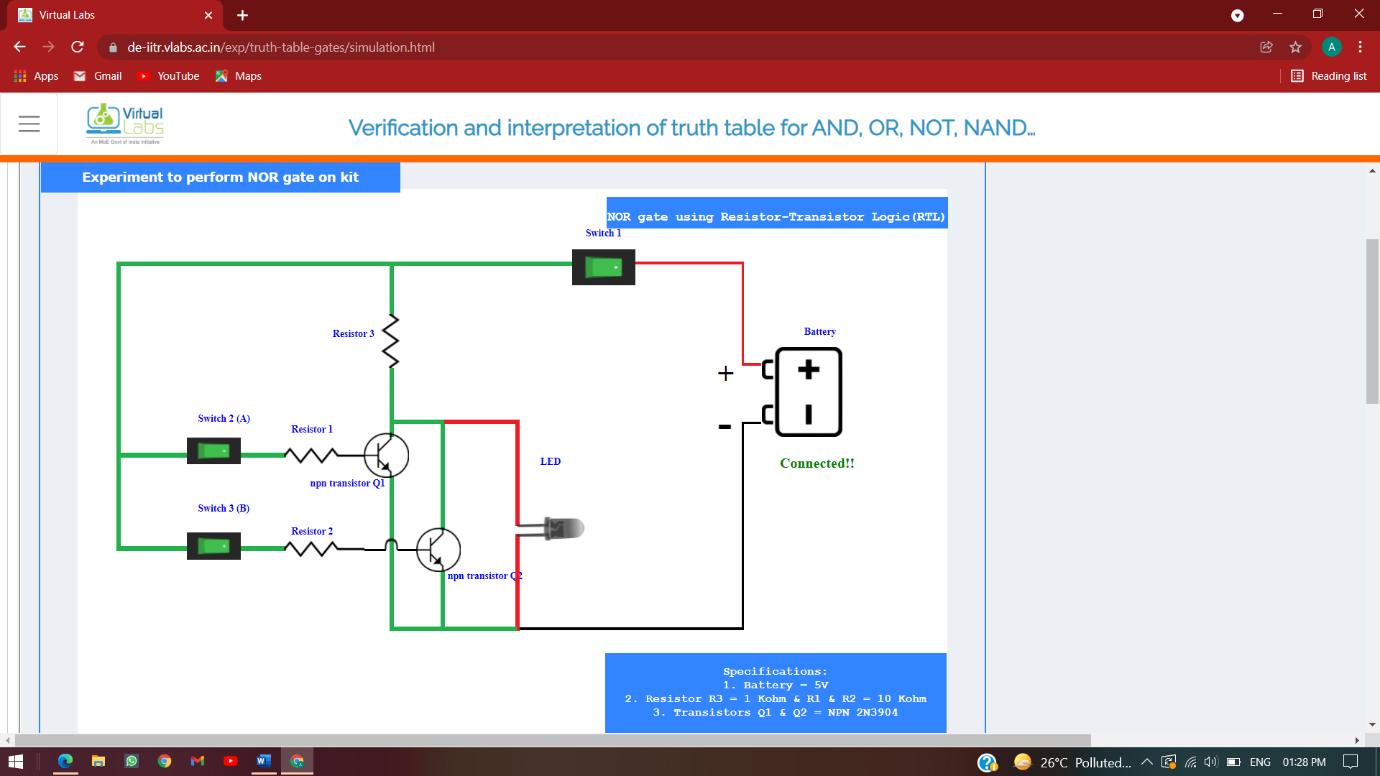
\includegraphics[width=0.9\linewidth]{img/exp5/6}
		\caption{}
		\label{fig:5:6}
	\end{figure}
		\begin{figure}[h]
		\centering
		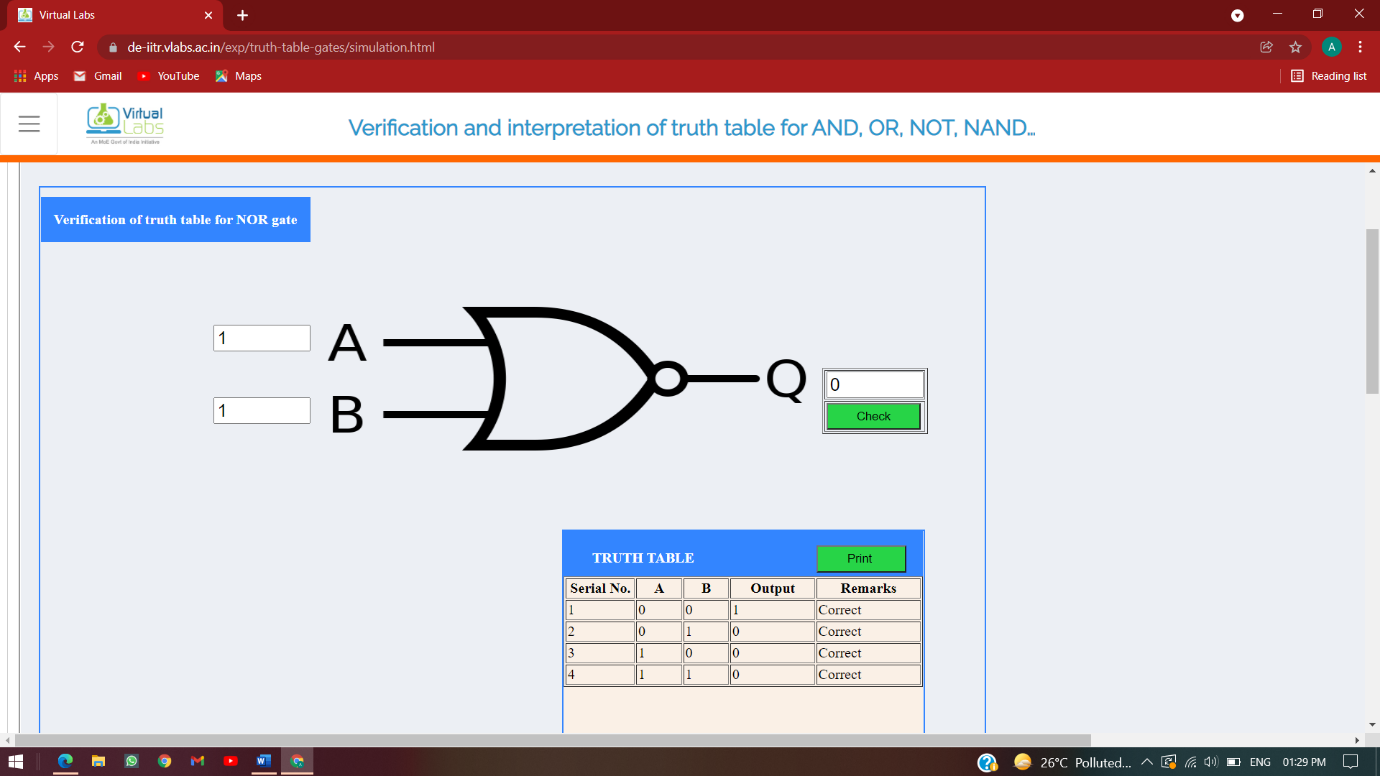
\includegraphics[width=0.9\linewidth]{img/exp5/7}
		\caption{}
		\label{fig:5:7}
	\end{figure}

\section{Conclusion}
NOR gate basically negates the results of OR gate . The output is low when both the inputs are high or when even one of the input is low. Iff both the inputs are low, we get a high output.

\section{Precautions}
	\begin{enumerate}
		\tightlist
		\item Make the connections when power supply is OFF.
		\item Ensure that the connections are tight.
		\item Change the status of inputs only when power supply is OFF.
	\end{enumerate}